\def\CTeXPreproc{Created by ctex v0.2.12, don't edit!}\documentclass{beamer}
\usepackage{graphicx}
\usepackage{verbatim}
\usepackage{amsmath}
\usepackage{amsfonts}
\usepackage{setspace}
% \usepackage{beamerthemesplit} // Activate for custom appearance

\title{Inference in Normal Regression Model}
\author{Dr. Frank Wood}

\date{}

\DeclareMathOperator*{\Ave}{\mathbb{E}}
\DeclareMathOperator*{\Var}{Var}

\begin{document}

\frame{\titlepage}



\frame[t] {
 \frametitle{Remember}
\begin{enumerate}
\item Last class we derived the sampling variance of the estimator of the slope, it being
$$\sigma^2\{b_1\} = \frac{\sigma^2}{\sum(X_i - \bar X)^2}$$
\item And we made the point that an estimate of $\Var(b_1)$ could be arrived at by substituting the MSE for the unknown error variance.
$$s^2\{b_1\} = \frac{MSE}{\sum(X_i - \bar X)^2} = \frac{\frac{SSE}{n-2}}{\sum(X_i - \bar X)^2}$$
\end{enumerate}
}

\frame[t] {
 \frametitle{Sampling Distribution of $(b_1 - \beta_1)/s(b_1)$}
\begin{enumerate}
\item We determined that $b_1$ is normally distributed so $(b_1 - \beta_1)/\sigma(b_1)$ is a standard normal variable
\item We don't know $\Var(b_1)$ so it must be estimated from data.  We have already denoted it's estimate
$s(b_1)$
\item Using this estimate we it can be shown that
$$\frac{b_1-\beta_1}{s\{b_1\}} \sim t(n-2)$$
$$s\{b_1\} = \sqrt{ s^2\{b_1\}}$$
\end{enumerate}
}

\frame[t] {
 \frametitle{Where does this come from?}
\begin{enumerate}
\item We need to rely upon the following theorem\\
For the normal error regression model
$$\frac{SSE}{\sigma^2} = \frac{\sum (Y_i - \hat Y_i)^2}{\sigma^2} \sim \chi^2(n-2)$$
and is independent of b0 and b1
\item Intuitively this follows the standard result for the sum of squared normal random variables
\\Here there are two linear constraints imposed by the regression
parameter estimation that each reduce the number of degrees of
freedom by one.
\end{enumerate}
}

\frame[t] {
 \frametitle{Another useful fact : t distribution}
Let z and $\chi^2(\nu)$ be independent random variables (standard
normal and $\chi^2$ respectively).  We then define a t random
variable as follows:
$$t(\nu) = \frac{z}{\sqrt{\frac{\chi^2(\nu)}{\nu}}}$$
This version of the t distribution has one parameter, the degrees of
freedom $\nu$

}

\frame[t] {
 \frametitle{Distribution of the studentized statistic}
To derive the distribution of this statistic, first we do the
following rewrite
$$\frac{b_1 - \beta_1}{{\hat S(b_1)}} = \frac{\frac{b_1 - \beta_1}{{ S(b_1)}}}{\frac{\hat S(b_1)}{ S(b_1)}}$$
$$\frac{\hat S(b_1)}{ S(b_1)} = \sqrt{\frac{\hat V(b_1)}{ V(b_1)}}$$}

\frame[t] {
 \frametitle{Studentized statistic cont.}
And note the following
$$\frac{\hat V(b_1)}{ V(b_1)} = \frac{\frac{MSE}{\sum(X_i-\bar X)^2}}{\frac{\sigma^2}{\sum(X_i-\bar X)^2}} = \frac{MSE}{\sigma^2} = \frac{SSE}{\sigma^2(n-2)}$$
where we know (by the given theorem) the distribution of the last
term is $\chi^2$ and indep. of $b_1$ and $b_0$
$$\frac{SSE}{\sigma^2(n-2)} \sim \frac{\chi^2(n-2)}{n-2}$$}

\frame[t] {
 \frametitle{Studentized statistic final}
But by the given definition of the t distribution we have our result
$$\frac{b_1-\beta_1}{\hat{S}(b_1)} \sim t(n-2)$$
because putting everything together we can see that $$\frac{b_1 -
\beta_1}{\hat S(b_1)} \sim
\frac{z}{\sqrt{\frac{\chi^2(n-2)}{n-2}}}$$ }

\frame[t] {
 \frametitle{Confidence Intervals and Hypothesis Tests}
Now that we know the sampling distribution of $b_1$ (t with n-2
degrees of freedom) we can construct confidence intervals and
hypothesis tests easily }


\frame[t] {
 \frametitle{Confidence Interval for $\beta_1$}
Since the ``studentized'' statistic follows a t distribution we can
make the following probability statement
$$P(t(\alpha/2; n-2)  \leq \frac{b_1-\beta_1}{s\{b_1\}}  \leq t(1-\alpha/2; n-2) ) = 1- \alpha$$
\begin{figure}
  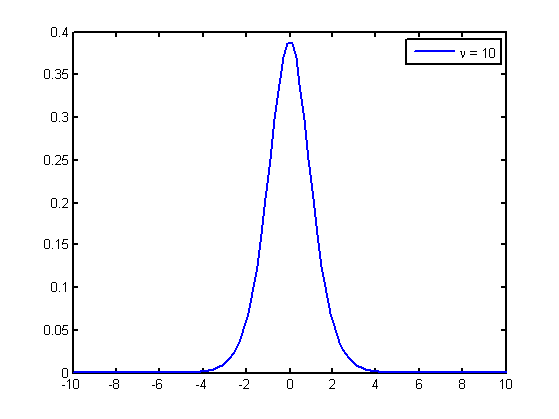
\includegraphics[height=20mm]{1.png}
  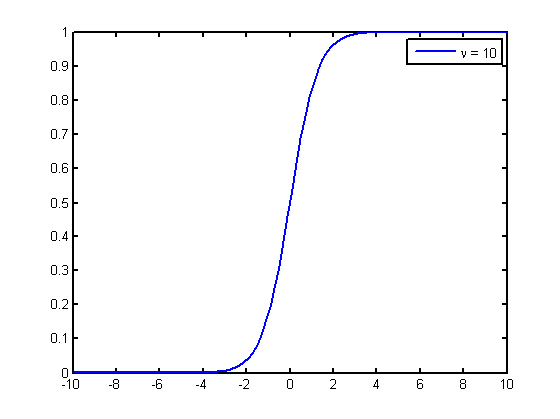
\includegraphics[height=20mm]{2.png}
  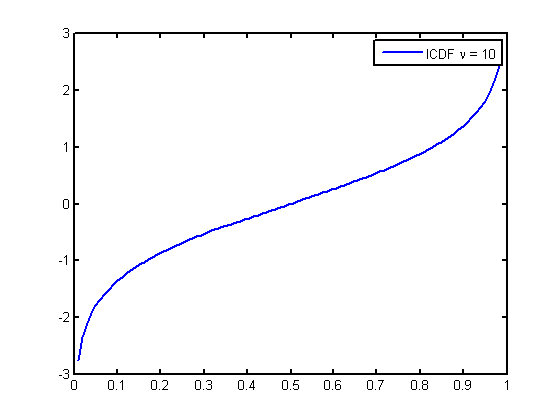
\includegraphics[height=20mm]{3.png}
\end{figure}}

\frame[t] {
 \frametitle{Interval arriving from picking $\alpha$}
\begin{enumerate}
\item Note that by symmetry $$t(\alpha/2; n-2) = -t(1-\alpha/2; n-2)$$
\item Rearranging terms and using this fact we have $$P(b_1 - t(1-\alpha/2; n-2 )s\{b_1\} \leq \beta_1  \leq b_1 + t(1-\alpha/2; n-2 ) s\{b_1\}) = 1- \alpha$$
\item And now we can use a table to look up and produce confidence intervals
\end{enumerate}
}

\frame[t] {
 \frametitle{Using tables for Computing Intervals }
\begin{enumerate}
\item The tables in the book (table B.2 in the appendix) for t(1-\alpha/2;\nu) where
$P\{t(\nu)\leq t(1-\alpha/2;\nu)\} = A$
\item Provides the inverse CDF of the t-distribution
\item This can be arrived at computationally as well\\
Matlab: $tinv(1-\alpha/2, \nu)$
\end{enumerate}
}

\frame[t] {
 \frametitle{$1-\alpha$ confidence limits for $\beta_1$}
\begin{enumerate}
\item The $1-\alpha$ confidence limits for $\beta_1$ are
$$b_1 \pm  t(1-\alpha/2; n-2 )s\{b_1\}$$
\item Note that this quantity can be used to calculate confidence intervals given n and \alpha.
\begin{enumerate}
\item Fixing $\alpha$ can guide the choice of sample size if a particular confidence interval is desired
\item Give a sample size, vice versa.
\end{enumerate}
\item Also useful for hypothesis testing
\end{enumerate}
}

\frame[t] {
 \frametitle{Tests Concerning $\beta_1$}
\begin{enumerate}
\item Example 1
\begin{enumerate}
\item Two-sided test
\begin{enumerate}
\item $H_0 : \beta_1 = 0$
\item $H_a : \beta_1 \neq 0$
\item Test statistic
$$t^* = \frac{b_1-0}{s\{b_1\} }$$
\end{enumerate}
\end{enumerate}
\end{enumerate}
}

\frame[t] {
 \frametitle{Tests Concerning $\beta_1$}
\begin{enumerate}
\item We have an estimate of the sampling distribution of $b_1$ from the data.
\item If the null hypothesis holds then the $b_1$ estimate coming from the data
should be within the $95\%$ confidence interval of the sampling
distribution centered at 0 (in this case)
$$t^* = \frac{b_1-0}{s\{b_1\} }$$
\end{enumerate}
}

\frame[t] {
 \frametitle{Decision rules}
\begin{eqnarray*}
\mathrm{if }\,  |t^*| &\leq& t(1-\alpha/2;n-2)\mathrm{, conclude } \, H_0\\
\mathrm{if }\,  |t^*| &>& t(1-\alpha/2;n-2)\mathrm{, conclude }\,
H_\alpha
\end{eqnarray*}
Absolute values make the test two-sided }

\frame[t] {
 \frametitle{Intuition}
\begin{figure}
  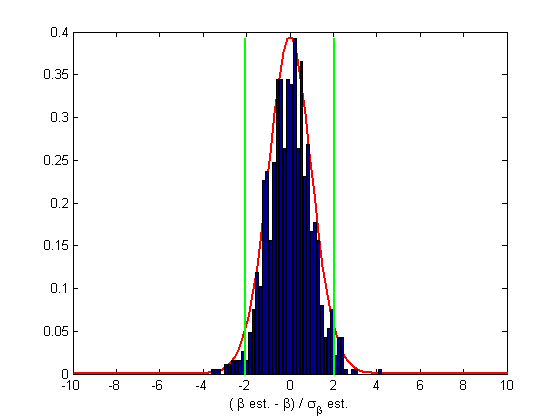
\includegraphics[height=60mm]{intuition.png}
\end{figure}
p-value is value of $\alpha$ that moves the green line to the blue
line }

\frame[t] {
 \frametitle{Calculating the p-value}
\begin{enumerate}
\item The p-value, or attained significance level, is the smallest level of significance $\alpha$
for which the observed data indicate that the null hypothesis should be rejected.
\item This can be looked up using the CDF of the test statistic.
\item In Matlab\\
Two-sided p-value\\
$2*(1-tcdf(|t^*|,\nu))$

\end{enumerate}
}

\frame[t] {
 \frametitle{Inferences Concerning $\beta_0$}
\begin{enumerate}
\item Largely, inference procedures regarding $\beta_0$ can be performed in the same way as those
for $\beta_1$
\item Remember the point estimator $b_0$ for $\beta_0$
$$b_0 = \bar Y - b_1 \bar X$$
\end{enumerate}
}

\frame[t] {
 \frametitle{Sampling distribution of $b_0$}
\begin{enumerate}
\item The sampling distribution of $b_0$ refers to the different values of $b_0$
that would be obtained with repeated sampling when the levels of the
predictor variable X are held constant from sample to sample.
\item For the normal regression model the sampling distribution of $b_0$ is normal

\end{enumerate}
}

\frame[t] {
 \frametitle{Sampling distribution of $b_0$}
\begin{enumerate}
\item When error variance is known
$$E(b_0) = \beta_0$$
$$\sigma^2\{b_0\} = \sigma^2 (\frac{1}{n} + \frac{\bar X^2}{\sum(X_i - \bar X)^2})$$
\item When error variance is unknown
$$s^2\{b_0\}= MSE (\frac{1}{n} + \frac{\bar X^2}{\sum(X_i - \bar
X)^2})$$
\end{enumerate}
}

\frame[t] {
 \frametitle{Confidence interval for $\beta_0$}
The $1-\alpha$ confidence limits for $\beta_0$ are obtained in the
same manner as those for $\beta_1$
$$b_0 \pm  t(1-\alpha/2; n-2 )s\{b_0\}$$
}

\frame[t] {
 \frametitle{Considerations on Inferences on $\beta_0$ and $\beta_1$}
\begin{enumerate}
\item Effects of departures from normality\\
The estimators of $\beta_0$ and $\beta_1$ have the property of
asymptotic normality - their distributions approach normality as the
sample size increases (under general conditions)
\item Spacing of the X levels
The variances of $b_0$ and $b_1$ (for a given n and $\sigma^2$)
depend strongly on the spacing of X

\end{enumerate}
}

\frame[t] {
 \frametitle{Sampling distribution of point estimator of mean response}
\begin{enumerate}
\item Let $X_h$ be the level of X for which we would like an estimate of the mean
response\\
Needs to be one of the observed X's
\item The mean response when $X=X_h$ is denoted by $\Ave(Y_h)$
\item The point estimator of $\Ave(Y_h)$ is
$$\hat Y_h = b_0 + b_1 X_h$$
We are interested in the sampling distribution of this quantity
\end{enumerate}
}

\frame[t] {
 \frametitle{Sampling Distribution of $\hat Y_h$}
\begin{enumerate}
\item We have
$$\hat Y_h = b_0 + b_1 X_h$$
\item Since this quantity is itself a linear combination of the $Y_i's$ it's sampling distribution is itself normal.
\item The mean of the sampling distribution is $$E\{\hat Y_h\} = E\{b_0\} + E\{b_1\} X_h = \beta_0 + \beta_1X_h$$
Biased or unbiased?
\end{enumerate}
}

\frame[t] {
 \frametitle{Sampling Distribution of $\hat Y_h$}
\begin{enumerate}
\item To derive the sampling distribution variance of the mean response we first show that
$b_1$ and $(1/n)\sum Y_i$ are uncorrelated and, hence, for the
normal error regression model independent
\item We start with the definitions
$$\bar Y = \sum (\frac{1}{n}) Y_i$$
\begin{eqnarray*}
b_1 &=& \sum k_i Y_i, \, k_i = \frac{(X_i - \bar X)}{\sum(X_i-\bar
X)^2}
\end{eqnarray*}

\end{enumerate}
}

\frame[t] {
 \frametitle{Sampling Distribution of $\hat Y_h$}
\begin{enumerate}
\item We want to show that mean response and the estimate $b_1$ are uncorrelated
$$Cov(\bar Y, b_1) = \sigma^2\{\bar Y, b_1\} = 0$$
\item To do this we need the following result (A.32)
$$\sigma^2\{\sum_{i=1}^n a_i Y_i, \sum_{i=1}^n c_i Y_i\} = \sum_{i=1}^n a_i c_i \sigma^2\{Y_i\}$$
when the $Y_i$ are independent
\end{enumerate}
}


\frame[t] {
 \frametitle{}

}

\frame[t] {
 \frametitle{}

}

\frame[t] {
 \frametitle{}

}

\frame[t] {
 \frametitle{}

}

\frame[t] {
 \frametitle{}

}

\frame[t] {
 \frametitle{}

}

\frame[t] {
 \frametitle{}

}

\frame[t] {
 \frametitle{}

}

\frame[t] {
 \frametitle{}

}

\frame[t] {
 \frametitle{}

}

\frame[t] {
 \frametitle{}

}

\frame[t] {
 \frametitle{}

}

\frame[t] {
 \frametitle{}

}

\frame[t] {
 \frametitle{}

}

\frame[t] {
 \frametitle{}

}

\frame[t] {
 \frametitle{}

}

\frame[t] {
 \frametitle{}

}

\frame[t] {
 \frametitle{}

}

\frame[t] {
 \frametitle{}

}

\frame[t] {
 \frametitle{}

}

\frame[t] {
 \frametitle{}

}

\frame[t] {
 \frametitle{}

}

\frame[t] {
 \frametitle{}

}

\end{document}
